

\chapter{Week 2: 29\textsuperscript{th} Sep - 5\textsuperscript{th} Oct}

\tocless\section{Objectives}

\begin{itemize*}
	\item Understand/Derive  Euler angles matrix
	\item Read up on datasheets for the 9DOF and the I2C protocol
\end{itemize*}

\tocless\section{Research Carried out}

\tocless\subsection{Derivation of Euler angle matrix}
Last week the rotation matrix was defined using \eqref{eq: rotation matrix}. If  this is solved for a Euler rotation of {\bf XYZ} one will get the following

\begin{align}
	\gls{rotationmatrix}(\gls{roll},\gls{pitch} ,\gls{yaw})
	 & = 	\overbrace{\begin{bmatrix}																
			1 & 0               & 0              \\
			0 & C_{\gls{roll}}  & S_{\gls{roll}} \\
			0 & -S_{\gls{roll}} & C_{\gls{roll}}
		\end{bmatrix}}^{\text{C}} 
	\overbrace{\begin{bmatrix}
			C_{\gls{pitch}} & 0 & -S_{\gls{pitch}} \\
			0               & 1 & 0                \\
			S_{\gls{pitch}} & 0 & C_{\gls{pitch} }
		\end{bmatrix}}^{\text{B}} 	
	\overbrace{\begin{bmatrix}
			C_{\gls{yaw}}   & S_{\gls{yaw}} & 0  \\
			- S_{\gls{yaw}} & C_{\gls{yaw}} & 0  \\
			0               & 0             & 1 
		\end{bmatrix}}^{\text{A}} \label{eq: rotation matrix solved} \\  	
	 & =  \begin{bmatrix}
		C_{\gls{pitch}}	C_{\gls{yaw}}                                              & C_{\gls{pitch}} S_{\gls{yaw}}                                             & -S_{\gls{pitch}}               \\
		S_{\gls{roll}}S_{\gls{pitch}}C_{\gls{yaw}}  - C_{\gls{roll}}S_{\gls{yaw}} & S_{\gls{roll}}S_{\gls{pitch}}S_{\gls{yaw}}  + C_{\gls{roll}}C_{\gls{yaw}} & C_{\gls{pitch}}S_{\gls{roll}}  \\
		C_{\gls{roll}}S_{\gls{pitch}}C_{\gls{yaw}}  + S_{\gls{roll}}S_{\gls{yaw}} & C_{\gls{roll}}S_{\gls{pitch}}S_{\gls{yaw}}  - S_{\gls{roll}}C_{\gls{yaw}} & C_{\gls{pitch}}C_{\gls{roll}} 
	\end{bmatrix}
\end{align}

Now letting $\hat{e}_i$ be the $i^{th}$ unit vector, the function that maps an Euler angle vector to it's corresponding Euler angle Rates matrix, $E:  \mathbb{ R}^3 \rightarrow \mathbb{ R}^{3x3}$, is

\begin{equation}
	{\bf E}_{ijk}(\gls{pitch},\gls{roll},\gls{yaw}) = [{\bf R}_k(\gls{yaw})^T {\bf R}_j(\gls{pitch})^T \hat{\bf e}_i, {\bf R}_k(\gls{yaw})^T\hat{\bf e}_j, \hat{\bf e}_k]
\end{equation}

Using the notation in \eqref{eq: rotation matrix solved} one will get the following equation. 

\begin{equation}
	{\bf E}_{ijk}(\gls{pitch},\gls{roll},\gls{yaw}) = {\bf A}^T{\bf B}^T\hat{\bf e}_{\gls{roll}} +  {\bf A}^T\hat{\bf e}_{\gls{pitch}} + \hat{\bf e}_{\gls{yaw}} 
	\label{eq: Euler angle matrix formula}
\end{equation}

After one has solved \eqref{eq: Euler angle matrix formula} for the Euler angle Rates matrix the angular velocity of the frame can then be found using the following.

\begin{equation}
	\omega = {\bf E}_{ijk}({\bf u}) \dot{\bf u}
	\label{eq: Angular velocity of the frame}
\end{equation}

\tocless\subsection{I\textsuperscript{2}C Protocol and SEN-10324 (9DOF)}

I\textsuperscript{2}C most commonly uses 7 bit address. When one sends out an address one uses 8 bits; 7 bits are used to assign the address and the last bit is used to inform the slave if it is reading or writing. Note the read/write bit is the LSD (Least Significant Bit)

\begin{figure}[h]
	\centering
	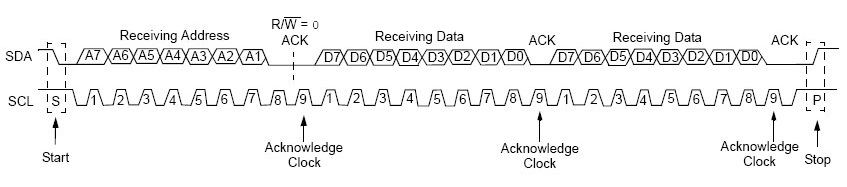
\includegraphics[width=1\linewidth]{\DocRoot/images/I2C_write}
	\caption{Typical I\textsuperscript{2}C write transmission (7-Bit Address)}
	
	\label{fig: I2C_write}
\end{figure}

When communicating with a device one will have to send a 8 bit packet. After the 8 bit a 9 bit is sent to acknowledge that the device has established a connection for communication. Note one can easily they if the master is reading from or writing to a device. If the 8 bit address is odd the master reading only and if the 8 bit address is even the writhing only.

\tocless\subsubsection{Writing to a Slave Device}
\begin{enumerate*}
	\item Send a start Sequence
	\item Send the I\textsuperscript{2}C address of the slave with R/W both low (even address)
	\item Send the internal register number one wants to write to.
	\item Send the data byte.
	\item{\bf Optional, send any further data bytes. }
	\item Send the stop sequence.
\end{enumerate*}

\newpage 

\tocless\subsubsection{Reading from Slave Device}
\begin{enumerate*}
	\item Send a start Sequence
	\item Send 0x53 ( I\textsuperscript{2}C address of the ADXL345 (accelerometer) with the R/W bit low (even address)
	\item Send 0x00  (Internal address used for device ID check )
	\item Send a start sequence again (repeated start)
	\item Send 0x53  ( I\textsuperscript{2}C address of the ADXL345  with the R/W bit high (odd address)
	\item Read data byte from ADXL345
	\item Send the stop sequence.
\end{enumerate*}

The 9DOF used in this project\footnote{\url{https://www.sparkfun.com/products/10724}} uses an accelerometer by Analog Devices  a digital Magnetometer by Honeywell and a  gyroscope  by InvenSense.

\tocless\subsection{ADXL345 Accelerometer}
The I\textsuperscript{2}C address for this devices is Ox53 (followed by the R/$\bar{\mathrm{W}}$ bit). This translates to OxA6 for the write and OxA7 for a read (See page 10 of data sheet\footnote{\url{https://www.sparkfun.com/datasheets/Sensors/Accelerometer/ADXL345.pdf}}) 

\tocless\subsection{HMC5883L Magnetometer}
The I\textsuperscript{2}C address for this devices is Ox1E. This translates to Ox3C for write and Ox3D for a read (See page 17 of data sheet\footnote{\url{https://dlnmh9ip6v2uc.cloudfront.net/datasheets/Sensors/Magneto/HMC5883L-FDS.pdf}} ) 


\tocless\subsection {ITG-3200 Gyroscope}
The I\textsuperscript{2}C address of this device is Ox68 as the $\mathrm{A}_0$ is tied to ground. This translates to OxD0 for the write and OxD1 for a read (See page 18 of data sheet\footnote{\url{https://www.sparkfun.com/datasheets/Sensors/Gyro/PS-ITG-3200-00-01.4.pdf}} )